\documentclass[
	9pt,
	a4paper,
	% kosection,
	% footnote,
	% nobookmarks,
	% microtype,
	figtabcapt,
%	lwarp
]{oblivoir}

%%%%%%%%%%%%%%%%
% Front Matter %
%%%%%%%%%%%%%%%%

\setcounter{secnumdepth}{5} % section numbering depth


\usepackage[dvipsnames]{xcolor}

\usepackage{fapapersize}
\usefapapersize{*,*,30mm,*,35mm,*}
\definefageometry{default}{30mm,*,35mm,*}[\nopagecolor]
\definefageometry{test}{15mm,25mm,35mm,*}[\pagecolor{cyan!15}]


\usepackage{kotex-logo}

%for reference
\usepackage{hyperref}
\hypersetup{colorlinks=true, linkcolor=black, urlcolor=cyan}
\renewcommand{\figureautorefname}{그림~}
\renewcommand{\tableautorefname}{표~}
% \renewcommand{\sectionautorefname}{foobar}
% \renewcommand{\subsectionautorefname}{foobarbaz}

\usepackage{afterpage}
\usepackage{oblivoir-misc}
\usepackage{graphicx}
\usepackage{fancyvrb}

\usepackage{fontspec-xetex}
% \setmainhangulfont{NanumMyeongjo-YetHangul.ttf}

\usepackage{tabularx}


% for citaiton
% \usepackage{biblatex}
							% Declare packages

%%%%%%%%%%
% Title, Authors, Date %
%%%%%%%%%%

\title{\vspace{-4cm}디지털휴먼엔터테인먼트특론 과제 2}
\author{120220210 고재현}
\date{\today}

\begin{document}


%%%%%%%%%%%%%%%%%%%%%
% Table of Contents %
%%%%%%%%%%%%%%%%%%%%%
\maketitle

% \begin{abstract}
% 이 문서는 2022 인공지능개론(EEE4178) 과목의 설명서이다.

% \end{abstract}

\pagenumbering{roman}                           % Start page numbering in Roman numerals
% \tableofcontents*        						% Add table of contents
% \clearpage

%%%%%%%%%%%%%%%%%
% preliminaries %
%%%%%%%%%%%%%%%%%

\setcounter{table}{0}		                    % Reset table counter
\setcounter{figure}{0}		                    % Reset figure counter

%%%%%%%%%%%%%
% Main Text %
%%%%%%%%%%%%%

\pagenumbering{arabic}							% Start page numbering in Arabic numerals

\section{개요} \label{sec:overview}
디지털 엔터테인먼트 분야에서, VR 및 AR 기술은 중요한 산업 분야이다.
디스플레이 기술이 발전함에 따라, 해당 기술에서의 시각적 사용자 경험은 중대되고 있으나,
청각적 사용자 경험을 고려하지 않는다면, 사용자 경험의 완성도는 떨어질 수 밖에 없다.
예를 들어 VRchat과 같이 여러 사용자가 함께 대회를 나누는 경우, 칵테일 파티 문제가 발생할 수 있다.
칵테일 파티 문제는 시끄러운 환경에서 여러 명의 사람들이 대화를 나누는 상황에서, 자신이 듣고자 하는 말소리를 구분하기 어려워지는 현상을 의미한다.
이러한 문제를 해결하기 위해서는, 사용자가 원하는 방향의 소리만을 강화하는 기술이 필요하다.
이러한 기술을 \textbf{Directional Hearing} 라고 하며, 본 논문에서는 이러한 기술이 VR/AR 환경에서 적용되도록 경량화한 모델을 제안하려고 한다.
\begin{figure}[htbp]
	\centering
	\label{fig:directhear}
	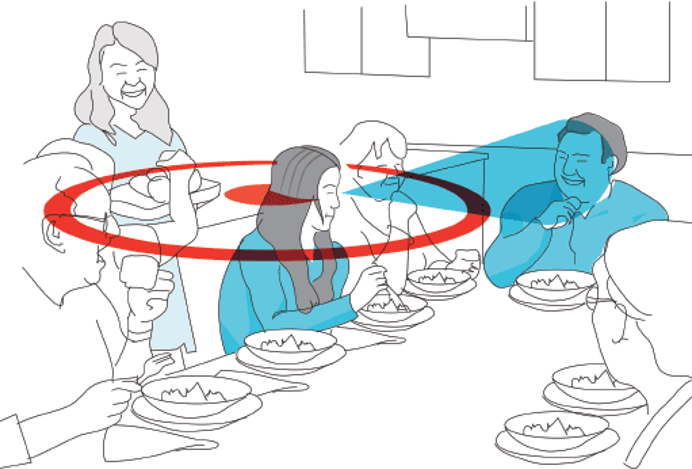
\includegraphics[width=0.5\linewidth]{figures/directhear.png}
	\caption{Directional Hearing Case}
\end{figure}
directional hearing의 상황은 그림 \ref{fig:directhear}과 같이 표현할 수 있다.

\section{latency requirements} \label{sec:latency}
\cite{stone1999tolerable}에서는 두 명의 화자가 대화를 나누되, 헤드셋을 통하여 소리를 전달하며 임의의 지연 시간을 추가하는 방법으로, 청력 기관이 허용하는 지연 시간의 한계를 추정하였다.
그 길이는 대략 20ms이다.
\cite{gupta2020acoustic} 에서도 AR 기기를 이용하여 유사한 실험을 진행하였는데, 같은 결과를 보였다.

청각적 사용자 경험뿐만 아니라, VR/AR 기기의 기능적 한계로 인해 20ms라는 요구사항을 맞추기 위해서는
\begin{itemize}
	\item 계산에 필요한 리소스는 줄이면서, Latency도 20ms 이내여야 하고
	\item 계산 능력이 떨어지는 단일 소스기기에서 처리 되어야 함
	\item 입력 소스는 Array mic 신호 및 각도 정보이며, 바라보는 방향의 소리를 분리 및 향상해야 한다.
\end{itemize}

\section{기존 연구} \label{sec:related}
지난 몇 년간, 이러한 문제를 해결하기 위한 다양한 연구들은 주로 Beamforming을 기반으로 진행되었다.~\cite{krim1996two, brayda2015spatially, chhetri2018multichannel}.
빔포밍과 같이 신호 처리를 기반으로 한 기술은 계산량이 적지만 성능이 원하는 만큼 높지 않다는 단점이 있다.
최근 연구들은 ~\cite{luo2019conv,jenrungrot2020cone} 딥러닝 기반의 기술들을 제안하여 Speech Separation 분야에서 뛰어난 성능을 보여주었다.
예를 들어 \cite[convTasNet]{luo2019conv}에서는 TCN, LN, MobileNet 등의 테크닉들을 활용하여 각 Speech Source에 대한 Mask를 추정하는 방식으로
Speech Separation 분야에서 뛰어난 성능을 보여주었다.

하지만, 딥러닝 기반의 기술들은 계산량이 많아 실시간 처리가 어렵거나, 모델의 크기가 커서 모바일 기기에서의 사용이 어렵다는 단점이 있다.


\subsection{HybridBeam} \label{sec:hybrid}
이 분야에서의 SOTA 모델은 AAAI 2022에 발표된 ~\cite[HybridBeam]{wang2021hybrid}이다.
HybridBeam은 빔포밍 기반의 전처리를 통해 딥러닝 모델의 연산량을 낮추는 방법으로 모델의 성능을 개선하였다.


\section{제안 방법} \label{sec:proposed}



\clearpage
%%%%%%%%%%%%%%%%%%%%%%
% References Section %
%%%%%%%%%%%%%%%%%%%%%%
\bibliographystyle{ieeetr}						% Declare bibliography style
\bibliography{ref.bib}							% Declare bibliography file

\clearpage

\end{document}
